\subsection{Лабораторный стенд}\label{section:secLabSetup}

Сиcтема считывания на основе платы PADIWA впервые использовалась на пучковых тестах CBM в ноябре~2014 г. Простейший анализ набранных данных показал, что некоторые распределения временных отметок не поддаются очевидному объяснению. В связи с этим потребовалось собрать лабораторный стенд, позволяющий более подробно исследовать особенности работы одного многоканального модуля системы считывания, описанного в разделе~\ref{section:secModule}. В некоторых измерениях выходной LVDS сигнал c PADIWA не оцифровывался ВПЦ, а считывался осциллографом с помощью активного зонда. Для лучшего понимания особенностей работы исследуемой системы считывания и сбора данных в том же лабораторном стенде был реализован более информативный, но медленный вариант системы считывания и сбора данных на основе 128-канальной микросхемы n-XYTER, каждый канал которой измеряет момент времени прихода переднего фронта и амплитуду входного сигнала. Эта система состоит из платы передней электроники 1xnxyter~\cite{}, подключаемой через печатную плату-адаптер к МА~ФЭУ и через контроллер считывания SysCore~ROC~\cite{SYSCORE} к ЭВМ. Для считывания одного МА~ФЭУ достаточно 64~каналов, то есть половины каналов одной платы передней электроники.

Схема лабораторного стенда приведена на \figref{fig:LabSetup}.

\begin{figure}[H]
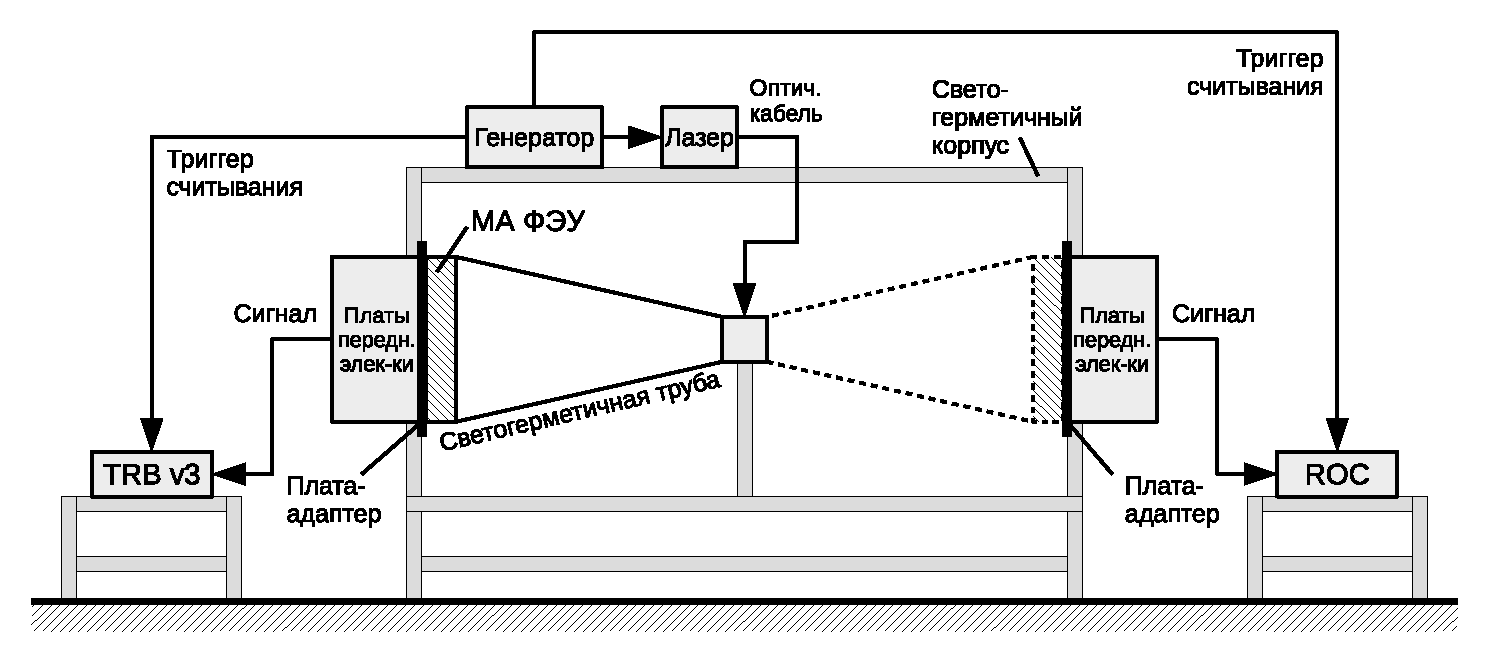
\includegraphics[width=1.0\textwidth]{pictures/12_Lab_setup_3_rus.eps}
\caption{Схема лабораторной установки.}
\label{fig:LabSetup}
\end{figure}

Стенд собран в светонепроницаемом корпусе размером 80~см на 80~см и длиной 2~м. В качестве источника света использовался такой же лазер Alphalas Picopower LD405~\cite{ALPHALAS} с поставляемым с ним генератором Alphalas PLDD-250~\cite{ALPHALAS}, как и в пучковых тестах. Свет от лазера поступал внутрь корпуса по оптоволокну.
% Пунктуация
Для того чтобы обеспечить равномерное освещение поверхности МА~ФЭУ свет лазера проходил через рассеивающее матовое стекло.
Интенсивность лазера подобрана так, чтобы каналы МА~ФЭУ работали в одноэлектронном режиме. Частота регистрации фотоэлектронов в каждом канале составляет около 10\% от частоты вспышек лазера.

На расстоянии приблизительно 30~см от рассеивающего стекла расположен МА~ФЭУ H12700. Для того чтобы обеспечить максимально чистые измерения, выполнена тщательная изоляция МА~ФЭУ от внешнего света. Рассеивающее стекло и МА~ФЭУ были помещены в черную, специально изготовленную на 3D~принтере, пластиковую трубу, которая, в свою очередь, была помещена в светоизолированный корпус.

Известно, что требуется некоторое время, чтобы МА~ФЭУ, находившийся на свету, высветился, поэтому перед началом измерений после закрытия корпуса обязательно выдерживался интервал не менее одного часа. В любой момент была возможность удалённо выключить лазер и исследовать темновой шум МА~ФЭУ. Для снижения наводок от люминесцентных ламп на время измерений свет в помещении выключался.

Две системы считывания и сбора данных были установлены одновременно, каждая на своей стороне корпуса. Упомянутая выше пластиковая труба, рассеивающее стекло и МА~ФЭУ поворачиваются как единое целое, обеспечивая одинаковые условия засветки МА~ФЭУ в положениях, соответствующих работе с обеими системами считывания.

Опорные печатные платы-адаптеры необходимы для того, чтобы на них с одной стороны крепились МА~ФЭУ, а с другой --- платы передней электроники. Плата-адаптер вмонтирована стенку коробки и выполняет роль каркаса и светоизолятора. Также по ней разведено питание МА~ФЭУ. Вся считывающая электроника питалась низким напряжением, а МА~ФЭУ высоким напряжением от высоковольтного источника.

Обе системы считывания и сбора данных являются самозапускающимися в том смысле, что каждый импульс на входе, при преодолении установленного порога, регистрируется и заносится в выходной буфер. Однако для того, чтобы данные из выходного буфера были отправлены в ЭВМ, необходимо периодически посылать во вспомогательный вход контроллера считывания специальный импульс, называемый триггером считывания. В нашей установке импульсы генератора, управляющего лазером, одновременно играют роль триггера считывания выходного буфера. В используемых системах считывания и сбора данных триггер считывания автоматически поступает во входной поток данных. Это позволяет анализировать зарегистрированные временные отметки, сопоставляя их с моментом вспышки лазера. Съём данных с обеих систем считывания и сбора данных осуществлялся по стандартному Ethernet кабелю в сетевой интерфейс ЭВМ.
